%%%%%%%%%%%%%%%%%%%%%%%%%%%%%%%%%%%%%%%%%%%%%%%%%%%%%%%%%%%%%%%%%%%%%%%%%%%%%%%
\section[Section]{Symmetric-key cryptography}
\part{Symmetric-key cryptography}

%%%%%%%%%%%%%%%%%%%%%%%%%%%%%%%%%%%%%%%%%%%%%%%%%%%%%%%%%%%%%%%%%%%%%%%%%%%%%%%
\begin{frame}{Symmetric-key cryptography}

  Symmetric ciphers are those where messages are encrypted and decrypted using the \textcolor{red}{same key}, which must be known only and exclusively to the two parts
  
  \medskip

  \phantom{padding}$\mathcal{C}(m, k) = c$ (encrypt function)
    
  \phantom{padding}$\mathcal{D}(c, k) = m$ (decrypt function)
  
  \medskip

  Obviously:
  
  \phantom{padding}$\mathcal{D}(\mathcal{C}(m, k), k) = m$ 
  
  \phantom{padding}The original message is \textcolor{red}{not altered} during the communication
  
  \medskip
  
  E.g. In the caesar cipher:
  
  \phantom{padding}$\mathcal{C}(m, k) = $ right shift of $k$ positions each character
  
  \phantom{padding}$\mathcal{D}(c, k) = $ left shift of $k$ positions each character

\end{frame}

%%%%%%%%%%%%%%%%%%%%%%%%%%%%%%%%%%%%%%%%%%%%%%%%%%%%%%%%%%%%%%%%%%%%%%%%%%%%%%%
\begin{frame}{Shannon principle}

  How to assess whether a cipher is robust enough? 
  
  (Where robustness means its probability of being successfully attacked)
  
  \medskip

  Shannon defines two key concepts:
  
  \begin{itemize}
    \item \textcolor{red}{Confusion}: the key must be well distributed in the encrypted message (each bit of the cipher should depend on each bit of the key with probability 50\%).
    \item \textcolor{red}{Diffusion}: the message must be well distributed in the encrypted message (each bit of the cipher should depend on each bit of the message with probability 50\%).
  \end{itemize}
  
  \medskip
  
  In the Caesar cipher we have no kind of diffusion and low confusion (why?)

\end{frame}

%%%%%%%%%%%%%%%%%%%%%%%%%%%%%%%%%%%%%%%%%%%%%%%%%%%%%%%%%%%%%%%%%%%%%%%%%%%%%%%
\begin{frame}{XOR cipher}

  Consider the \textcolor{red}{XOR} (exclusive or) operation $\oplus$, the following properties are valid:
  
  \begin{itemize}
    \item $0 \oplus 0 = 1 \oplus 1 = 0$ 
    \item $0 \oplus 1 = 1 \oplus 0 = 1$ 
    \item $x \oplus y \oplus y = x$ 
  \end{itemize}
  
  \medskip
  \pause
  
  We define the XOR cipher as:
    
  $\mathcal{C}(m, k) = m \oplus k$ \phantom{padding} ($m[i] \oplus k[i]$, $0 \leq i < ||m||$)
  
  $\mathcal{D}(c, k) = c \oplus k$ \phantom{padding} ($c[i] \oplus k[i]$, $0 \leq i < ||c||$)

  \medskip
  
  \pause

  Problem: the key $k$ could be \textcolor{red}{shorter} than the message $m$.
  
  Solution: reuse the key as $k^{'} = k \cdot k \cdot \ldots \cdot k$ until $||k^{'}||$ $m$.

  \medskip
  \pause
  
  Example:
  
  \texttt{m = 01100011 01101001 01100001 01101111} (ciao in ASCII).\\
  \texttt{k = 01111000 01111000 01111000 01111000} (x in ascii 4 times)\\
  \texttt{c = 00011011 00010001 00011001 00010111} (non printable, \texttt{GxEZFw==} in b64)
  
\end{frame}

%%%%%%%%%%%%%%%%%%%%%%%%%%%%%%%%%%%%%%%%%%%%%%%%%%%%%%%%%%%%%%%%%%%%%%%%%%%%%%%
\begin{frame}{One-time pad}

  \pause

  The problem with the XOR cipher is that encrypting repeatedly reusing the same key can leak \textcolor{red}{statistical informations} of the original message  
  
  \medskip
  
  We call Vernam cipher (or one-time pad) a XOR cipher where the key has the same length of the message. 
  
  \smallskip
  
  This cipher is called \textcolor{red}{perfect} because we have that:
  
  \medskip
  
  \phantom{pad}$P(M = m | C = c) = P(M = m)$
  
  \medskip
  
  The probability that $M$ is a certain message $m$ knowing that the cipher $C$ is $c$ is equal to the probability that $M$ is a certain message not knowing the cipher (all messages are equiprobable, the encrypted message does not give us any information about the real message).
  
  \medskip
  
  \pause

  Nice in theory, but:
  
  \begin{itemize}
    \item The key must be exchanged using a secure method (exchange them by \textit{hand}).
    \item The key must be generated randomly and not used (otherwise a many-time pad attack is possible).
  \end{itemize}

\end{frame}

%%%%%%%%%%%%%%%%%%%%%%%%%%%%%%%%%%%%%%%%%%%%%%%%%%%%%%%%%%%%%%%%%%%%%%%%%%%%%%%
\begin{frame}{Many-time pad \& XorTool}

  Nice article: 
  \textcolor{red}{\href{http://www.thecrowned.org/the-one-time-pad-and-the-many-time-pad-vulnerability}{thecrowned.org/the-one-time-pad-and-the-many-time-pad-vulnerability}}

  \smallskip
  
  \textcolor{red}{XorTool}: tool for statistical analysis of encrypted messages:

  \centerline{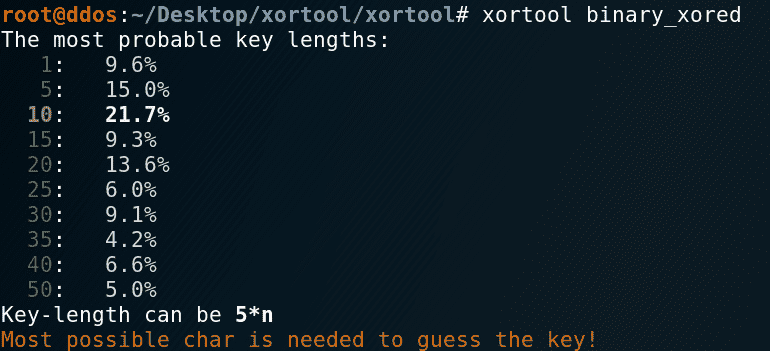
\includegraphics[width=5.5cm]{img/xortool}}

  \smallskip
  Knowing the initial part, we can see words in the message:
   
  \centerline{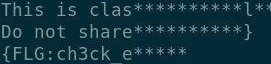
\includegraphics[width=4cm]{img/xor1}}

  Going by trial the final flag is reconstructed:
    
  \centerline{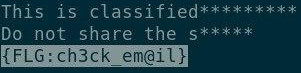
\includegraphics[width=4cm]{img/xor2}}


\end{frame}

%%%%%%%%%%%%%%%%%%%%%%%%%%%%%%%%%%%%%%%%%%%%%%%%%%%%%%%%%%%%%%%%%%%%%%%%%%%%%%%
\begin{frame}{Block vs Stream ciphers}

  \begin{columns}
  \begin{column}{0.5\textwidth}
    \textcolor{red}{Block ciphers}
    
    \begin{itemize}
      \item Works with fixed-length groups of bits (called blocks)
      \item More memory/time requirements
      \item High diffusion and confusion
      \item Error propagation
      \item Need to handle messages length (padding)
    \end{itemize}

    Famous ciphers:       \\
    \phantom{pad}DES      \\
    \phantom{pad}AES      \\
    \phantom{pad}BlowFish
  \end{column}
  \begin{column}{0.5\textwidth}
    \textcolor{red}{Stream ciphers}
    
    \begin{itemize}
      \item Works by encrypt digits one at the time
      \item Faster encryption/decryption
      \item Low diffusion
      \item Low propagation error
      \item Need a key stream (usually a shift register)
    \end{itemize}

    Famous ciphers:         \\
    \phantom{pad}ChaCha     \\
    \phantom{pad}Salsa20    \\
    \phantom{pad}LFSR-based
    
  \end{column}
  \end{columns}

\end{frame}

%%%%%%%%%%%%%%%%%%%%%%%%%%%%%%%%%%%%%%%%%%%%%%%%%%%%%%%%%%%%%%%%%%%%%%%%%%%%%%%
\begin{frame}{Padding a message (PKCS\#5 \& PKCS\#7)}

% \centering

How to handle messages of length not multiple of the block size?

\smallskip

Idea: append "some chars" to the message (\textcolor{red}{padding string})

\bigskip

\textcolor{red}{\textbf{PKCS\#5}}:

\textit{The padding string PS shall consist of $8 - (||M|| \mod 8)$ octets all having value $8 - (||M|| \mod 8).$}

\bigskip

\textcolor{red}{\textbf{PKCS\#7}}:

\textit{For such algorithms, the method shall be to pad the input at the trailing end with $k - (l \mod k)$ octets all having value $k - (l \mod k)$, where $l$ is the length of the input.}

\bigskip

Why $8 - (||M|| \mod 8)$ and not $(||M|| \mod 8)$?

\end{frame}

%%%%%%%%%%%%%%%%%%%%%%%%%%%%%%%%%%%%%%%%%%%%%%%%%%%%%%%%%%%%%%%%%%%%%%%%%%%%%%%
\begin{frame}{DES}

\textcolor{red}{D}ata \textcolor{red}{E}ncryption \textcolor{red}{S}tandard

Developed in 1975 by Feistel, encrypt blocks of 64 bits with a 56 bits key

Implements the confusion and diffusion principle by 16 rounds of the \textcolor{red}{Feistel function}

\medskip

  \begin{columns}
  \begin{column}{0.5\textwidth}
  
    \centerline{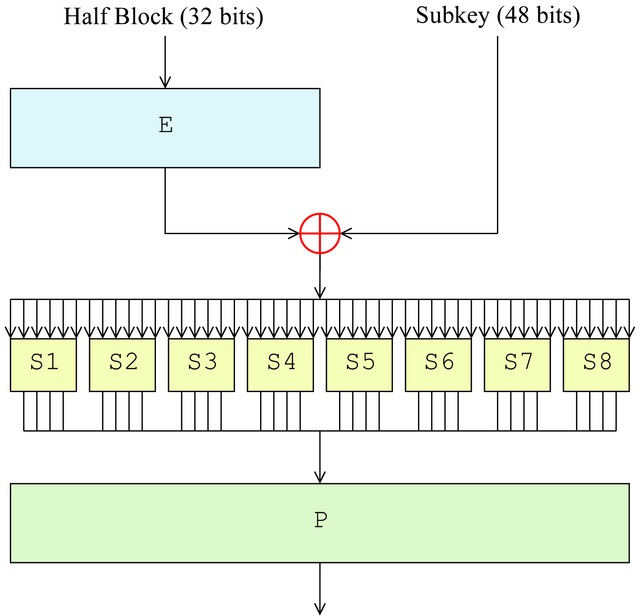
\includegraphics[width=5cm]{img/DES.png}}

  \end{column}
  \begin{column}{0.5\textwidth}
  
  The Feistel function consists in 4 stages:
  
  \begin{itemize}
    \item 1. \textcolor{red}{Expand} the half block from 32 to 48 bits (E-Box)
    \item 2. \textcolor{red}{Mix} result and subkey using a XOR operation
    \item 3. \textcolor{red}{Substitution} of the 6-bits input with a 4-bits output according to a lookup table (S-Box)
    \item 4. \textcolor{red}{Permutation} of the result (P-Box)
  \end{itemize}
    
  \end{column}
  \end{columns}

  \medskip

  Problem: DES vulnerable to a bruteforce attack (only 56 bits for the key...)
  
\end{frame}

%%%%%%%%%%%%%%%%%%%%%%%%%%%%%%%%%%%%%%%%%%%%%%%%%%%%%%%%%%%%%%%%%%%%%%%%%%%%%%%
\begin{frame}{AES}

\small

  \textcolor{red}{A}dvanced \textcolor{red}{E}ncryption \textcolor{red}{S}tandard

  \medskip

  AES replace DES starting from 2001 and is currently the standard in secure communications (TLS1.3 support only AES and ChaCha20)

  \medskip
  
  Based on a \textcolor{red}{substitution–permutation network} (equivalent of the Feistel network)

  \medskip
  
  \begin{columns}
  \begin{column}{0.25\textwidth}
    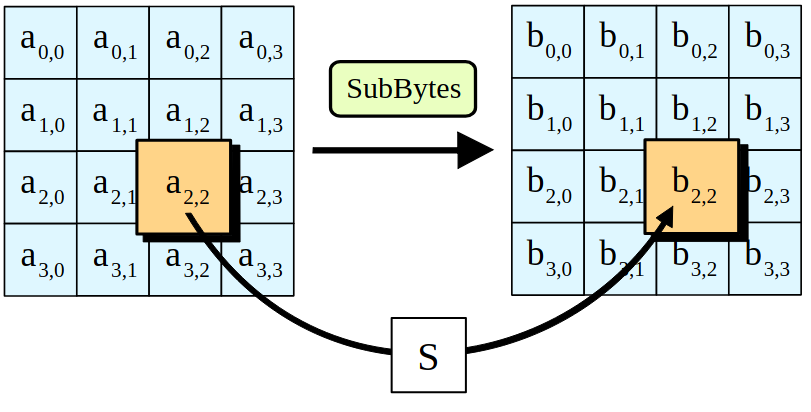
\includegraphics[width=3.5cm]{img/AES-1.png}
  \end{column}
  \begin{column}{0.25\textwidth}  
    Step 1: \\
    
    Each byte is replaced with another according to a lookup table (S-Box)
  \end{column}
  \begin{column}{0.25\textwidth}
    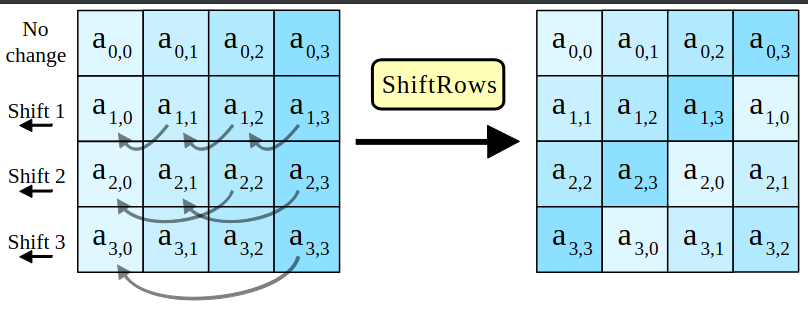
\includegraphics[width=3.5cm]{img/AES-2.png}
  \end{column}
  \begin{column}{0.25\textwidth}
    Step 2:\\
    
    Transposition of each rows by 0, 1, 2 or 3 positions
  \end{column}
  \end{columns}

  
  \begin{columns}
  \begin{column}{0.25\textwidth}
    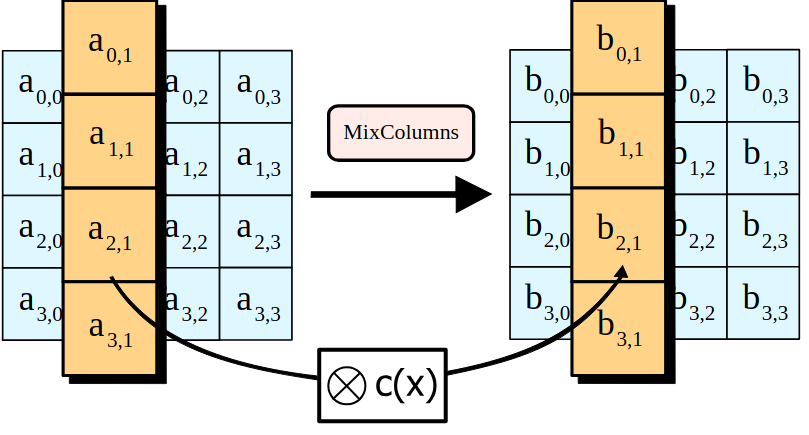
\includegraphics[width=3.5cm]{img/AES-3.png}
  \end{column}
  \begin{column}{0.25\textwidth}
    Step 3: \\
    
    Linear mixing operation where each column is mapped into a new one
  \end{column}
  \begin{column}{0.25\textwidth}
    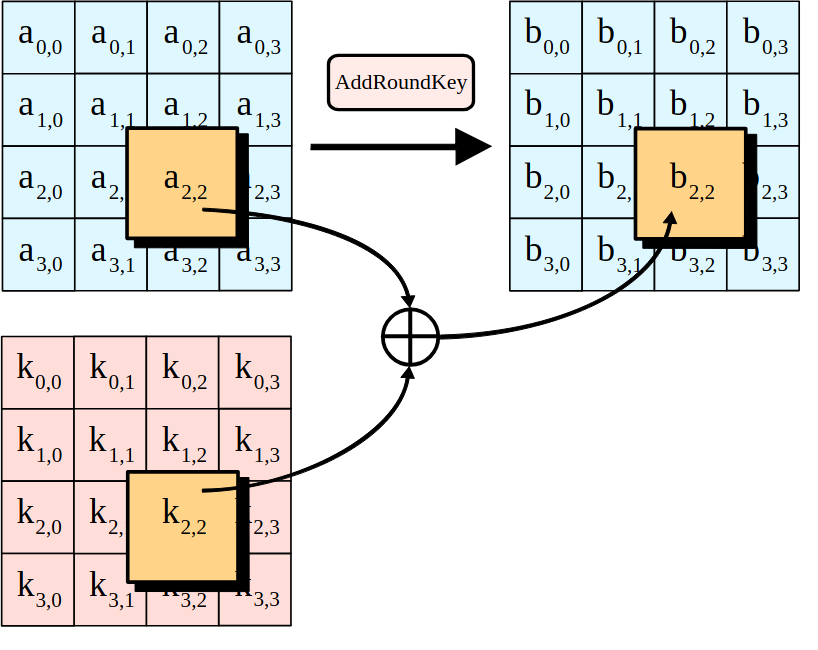
\includegraphics[width=3.5cm]{img/AES-4.png}
  \end{column}
  \begin{column}{0.25\textwidth}
    Step 4: \\
    
    Each byte is XORed with the corresponding value of the subkey
  \end{column}
  \end{columns}

\end{frame}

%%%%%%%%%%%%%%%%%%%%%%%%%%%%%%%%%%%%%%%%%%%%%%%%%%%%%%%%%%%%%%%%%%%%%%%%%%%%%%%
\begin{frame}{Block cipher mode of operation}

  How to ciphers two or more blocks? Different modes, different features:
  
  \begin{itemize}
    \item \textcolor{red}{Parallel encryption}: encrypt different blocks at the same time (without race conditions)
    \item \textcolor{red}{Parallel decryption}: decrypt different blocks at the same time (without race conditions)
    \item \textcolor{red}{Random read}: decrypt any single block without decrypting the previous ones
  \end{itemize}

\begin{table}[]
\begin{tabular}{|l|l|l|l|}
\hline
Mode                        & \begin{tabular}[c]{@{}l@{}}Parallel \\ encryption\end{tabular} & \begin{tabular}[c]{@{}l@{}}Paralllel \\ decryption\end{tabular} & \begin{tabular}[c]{@{}l@{}}Random\\ read\end{tabular} \\ \hline
\textcolor{red}{Electronic Code Book (ECB)}   & Yes                                                            & Yes                                                             & Yes                                                   \\ \hline
\textcolor{red}{Cipher Block Chaining (CBC)} & No                                                             & Yes                                                             & Yes                                                   \\ \hline
Propagating CBC (PCBC)      & No                                                             & No                                                              & No                                                    \\ \hline
Cipher Feedback (CFB)       & No                                                             & Yes                                                             & Yes                                                   \\ \hline
Output Feedback (OFB)       & No                                                             & No                                                              & No                                                    \\ \hline
Counter (CTR)               & Yes                                                            & Yes                                                             & Yes                                                   \\ \hline
\end{tabular}
\end{table}

\end{frame}

%%%%%%%%%%%%%%%%%%%%%%%%%%%%%%%%%%%%%%%%%%%%%%%%%%%%%%%%%%%%%%%%%%%%%%%%%%%%%%%
\begin{frame}{ECB (Electronic Code Book)}

The message is divided into blocks, and each block is encrypted/decrypted \textcolor{red}{separately}:

\medskip

\centerline{$C_i = f(M_i, Key)$}

\centerline{$M_i = f(C_i, Key)$}

\medskip

\centerline{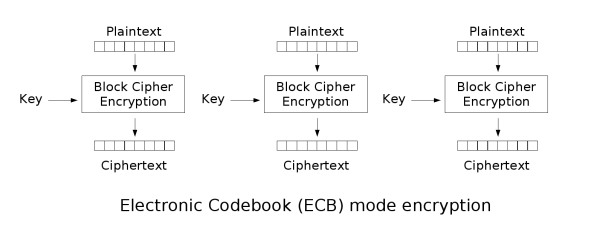
\includegraphics[width=9cm]{img/ECB.png}}

\medskip

Problem: \textcolor{red}{no diffusion}, ECB encrypt same plaintext in same ciphertext

\end{frame}

%%%%%%%%%%%%%%%%%%%%%%%%%%%%%%%%%%%%%%%%%%%%%%%%%%%%%%%%%%%%%%%%%%%%%%%%%%%%%%%
\begin{frame}{How to break ECB (padding-oracle attack)}

  \centerline{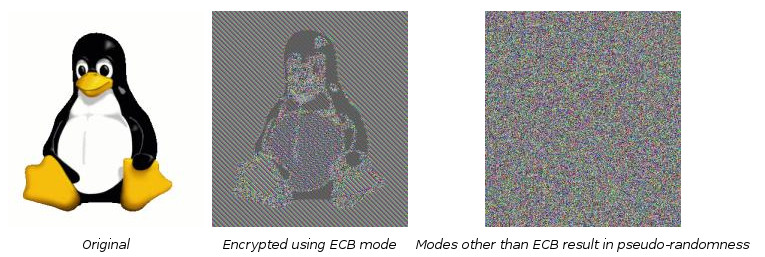
\includegraphics[width=9cm]{img/tux.jpg}}


\end{frame}

%%%%%%%%%%%%%%%%%%%%%%%%%%%%%%%%%%%%%%%%%%%%%%%%%%%%%%%%%%%%%%%%%%%%%%%%%%%%%%%
\begin{frame}{CBC (Cipher Block Chaining)}

In CBC each block of plaintext is XORed with the \textcolor{red}{previous ciphertext} block before being encrypted. An initialization vector in needed for the first block.
 
\medskip

\centerline{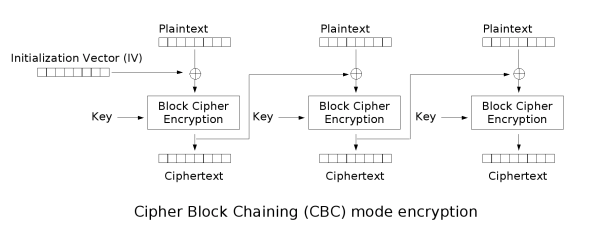
\includegraphics[width=9cm]{img/CBC.png}}

\medskip

\phantom{pad}$C_0 = IV$

\phantom{pad}$C_{i+1} = \mathcal{C}(M_i \oplus C_{i}, Key)$

\phantom{pad}$M_{i+1} = \mathcal{D}(C_{i+1}, Key) \oplus C_{i}$
\end{frame}

%%%%%%%%%%%%%%%%%%%%%%%%%%%%%%%%%%%%%%%%%%%%%%%%%%%%%%%%%%%%%%%%%%%%%%%%%%%%%%%
%\begin{frame}{How to break CBC (bit-flipping attack)}

%\end{frame}

%%%%%%%%%%%%%%%%%%%%%%%%%%%%%%%%%%%%%%%%%%%%%%%%%%%%%%%%%%%%%%%%%%%%%%%%%%%%%%%
\begin{frame}{Stream cipher: LFSR}

  \textcolor{red}{L}inear-\textcolor{red}{F}eedback \textcolor{red}{S}hift \textcolor{red}{R}egisters
  
  \medskip

  Shift register whose input bit is a linear function of its previous state
   
  \medskip
  
  \begin{columns}
  \begin{column}{0.5\textwidth}
    \centerline{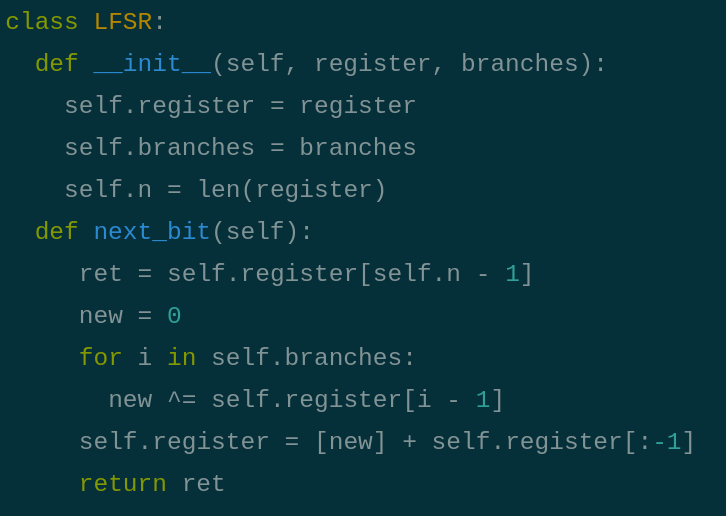
\includegraphics[width=6cm]{img/LFSR-code.png}}
  \end{column}
  \begin{column}{0.5\textwidth}
    \centerline{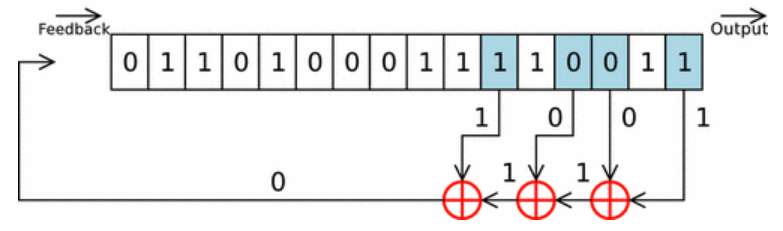
\includegraphics[width=6cm]{img/lfsr.png}}

    \medskip

    \centerline{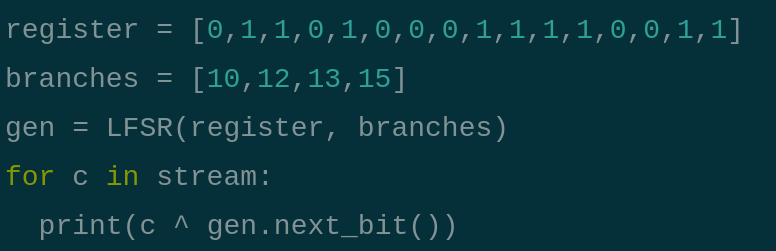
\includegraphics[width=6cm]{img/LFSR-gen.png}}
  \end{column}
  \end{columns}

\end{frame}
